\marginnote{This subsection is intended for readers who are not already familiar with the power system. It clarifies basic concepts such as production/consumption balance, system frequency, system operators, energy markets, etc.}
The goal of the power system is to provide an adequate and secure electricity supply to the population.
The electric power system today is composed of two layers (Figures~\ref{fig:powernow}-\ref{fig:marketnow}): 
\begin{description}
	\item[Physical grid] This is the level at which the electricity flows, going from generators to transmission system, to distribution system and finally to the end consumer.
	\item[Market layer] This is where all the energy trade and business operations are made. This includes the sale of electricity from producers to \glspl{brc}. Retailers in turn buy electricity from the BRCs and sell it to the end consumer. Being a \gls{brp}, either as a consumer or as a producer, means that the actor is responsible for its own forecasts and must ensure the best possible that the actual production/consumption follows the planned schedules.
\end{description}

\begin{figure}[t]
	\centering
	\caption{The Electric Power System as seen today. The power generated is first transmitted at high voltage levels to industrial consumers and transformer substations, from where it is distributed at medium/low voltage to medium size consumers and households.}\label{fig:powernow}
	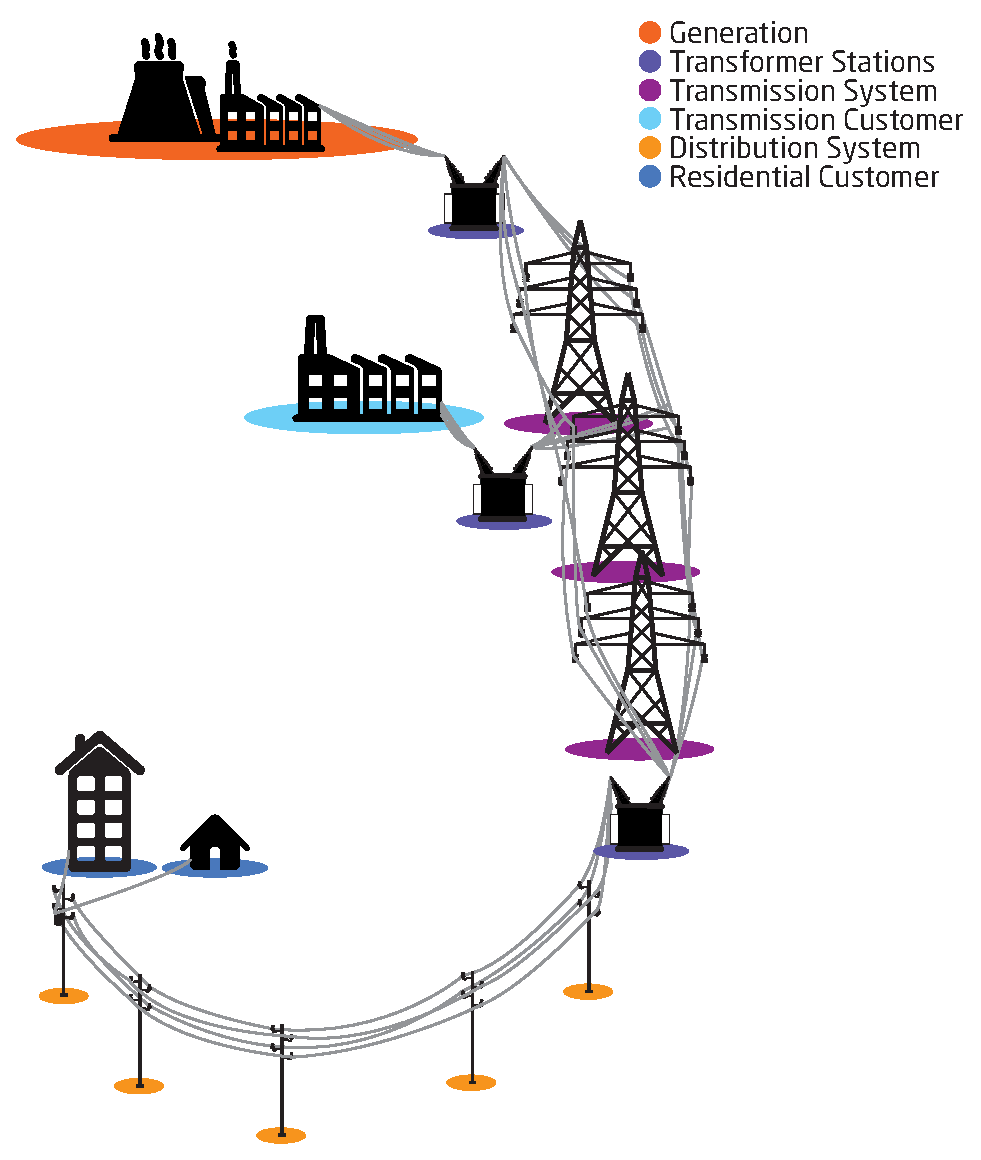
\includegraphics[width=\textwidth]{intro/traditional_grid_new.eps}
\end{figure}

While market regulations can be adjusted or completely changed in order to cope with the large influx of renewable energy, the physical laws cannot.
When electricity is produced it must also be consumed. With current technology it is unfeasible to store electricity in large quantities, therefore electricity companies must forecast how much electricity consumers are going to need the next day and then buy electricity accordingly. I.e., the production of electricity must match the consumption of electricity. If there is a surplus of electricity in the system (production exceeds consumption), the system frequency increases\sidenote[][-3\baselineskip]{The system frequency is a measure of the balance of the grid. Electricity is traditionally produced with turbines which rotate synchronously in a given area. The system frequency, e.g. 50 Hz in Europe, is a measure of the balance of the system, with higher frequencies signaling a power surplus and lower frequencies signaling power deficit in the system.}%\todo{Check up on sources}}
, and might eventually damage electric components in the grid. Vice versa, a deficiency of electricity in the system (consumption exceeds production) can lead to a blackout. 
\begin{figure*}[htbp!]
		\centering
		\caption{The actors and relationships in the power market today. Note that the consumer buys electricity from a retailer, but has no further contact to the other market actors, i.e. the consumer has a passive role in the system.}\label{fig:marketnow}
	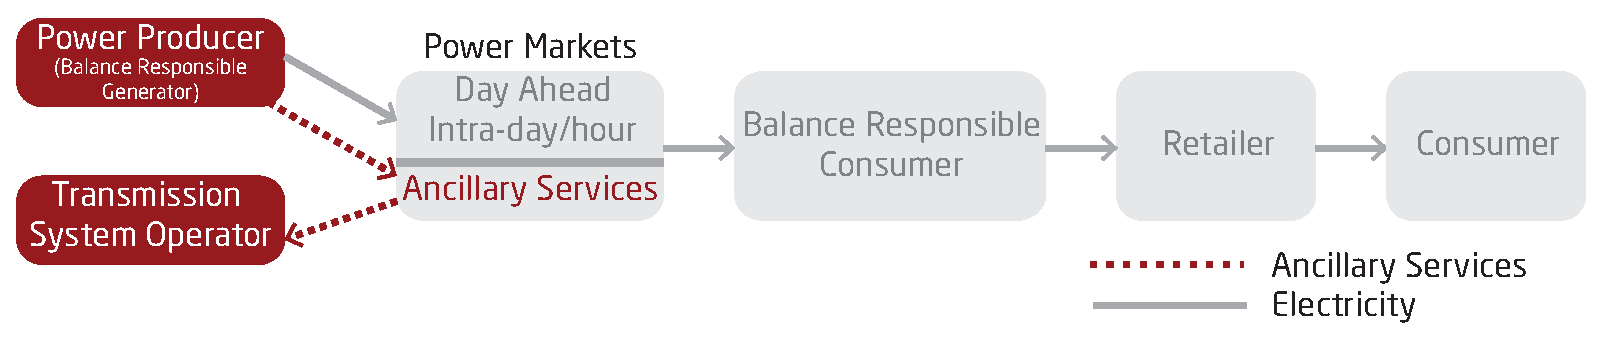
\includegraphics[width=\textwidth]{intro/market_now.eps}
\end{figure*}

The consumption forecasts are imperfect, which leads to a constant imbalance between production and consumption of electricity. The \gls{tso} is the entity responsible of resolving the imbalances of the system and maintaining the secure operation of the system. In order to do this, the TSO buys ancillary services from \emph{certified generators}\footnote[][-2\baselineskip]{The concept of certification of units to deliver ancillary services is central to this work and will be expanded upon in Chapter~\ref{cha:validation}.}  through the ancillary service markets. This market relationship is also reflected in Figure~\ref{fig:marketnow}. There are different types of services, and thorough overviews and explanations of these can be found in the literature\fcite{entso1operational,Rebours}. Here it suffices to say\footnote{Further discussion on ancillary services will be presented in Chapter~\ref{cha:services}.} that for most ancillary services, the TSO will pay generators to deviate from their planned production plans in order to bring the system back to balance. In the future, it is expected that the traditional sources of ancillary services, i.e. large central fossil-fuel powered generation plants, will be outphased in favor of smaller distributed and renewable generation. This means that new sources for ancillary services must be found.  
